\documentclass[aspectratio=169, 10pt]{beamer}

\usepackage{bm} % bold math
\usepackage{fontspec}
\usepackage{minted}
\usepackage{pgf-pie}
\usepackage{tikz}
\usepackage{graphicx}
\newcommand\sbullet[1][.5]{\mathbin{\vcenter{\hbox{\scalebox{#1}{$\bullet$}}}}}

% Custom commands and environments
\makeatletter
\newcommand\version[1]{\renewcommand\@version{#1}}
\newcommand\@version{}
\def\insertversion{\@version}

\newcommand\course[1]{\renewcommand\@course{#1}}
\newcommand\@course{}
\def\insertcourse{\@course}

\newcommand\coursetitle[1]{\renewcommand\@coursetitle{#1}}
\newcommand\@coursetitle{}
\def\insertcoursetitle{\@coursetitle}

\newcommand\lecturenumber[1]{\renewcommand\@lecturenumber{#1}}
\newcommand\@lecturenumber{}
\def\insertlecturenumber{\@lecturenumber}
\makeatother

\newcommand{\slidetitle}[1]{{\xbseries \large \structure{#1}} \bigskip}
\newcommand{\term}[1]{{\color{blue} #1}}
\newcommand{\leftspace}{\hspace{1em}}
\newcommand{\inlinearrow}{
  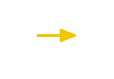
\begin{tikzpicture}[baseline]
    \node [anchor=base] (x) {};
    \draw [rawarrow] (x.mid west) -- ($(x.mid west) + (2em,0)$);
  \end{tikzpicture}
}

\newenvironment{slide}
{\begin{frame}[fragile,environment=slide]\vskip0pt plus 1filll}
{\vskip0pt plus 1filll\end{frame}}

% LaTeX

\setlength{\leftmargini}{1em}

% Common Information

\author{Talia Xu}
\course{COMPSCI 340}
\coursetitle{Operating Systems}
\date{2024 Semester 2}

% fontspec

\defaultfontfeatures{Ligatures=TeX}
% \setmainfont{Domine}
\setsansfont{Inter}[
  FontFace={ul}{n}{Font=*-Thin},
  FontFace={el}{n}{Font=*-ExtraLight},
  FontFace={l}{n}{Font=*-Light},
  FontFace={sb}{n}{Font=*-SemiBold},
  FontFace={eb}{n}{Font=*-ExtraBold},
  FontFace={xb}{n}{Font=*-Black},
]
\setmonofont[Contextuals=AlternateOff, Ligatures=TeXOff]{Iosevka}[
  FontFace={xb}{n}{Font=*-Heavy},
]

%% Font Weights

\DeclareRobustCommand{\ulseries}{\fontseries{ul}\selectfont}
\DeclareTextFontCommand{\textul}{\ulseries}
\DeclareRobustCommand{\elseries}{\fontseries{el}\selectfont}
\DeclareTextFontCommand{\textel}{\elseries}
\DeclareRobustCommand{\lseries}{\fontseries{l}\selectfont}
\DeclareTextFontCommand{\textl}{\lseries}
\DeclareRobustCommand{\sbseries}{\fontseries{sb}\selectfont}
\DeclareTextFontCommand{\textsb}{\sbseries}
\DeclareRobustCommand{\ebseries}{\fontseries{eb}\selectfont}
\DeclareTextFontCommand{\texteb}{\ebseries}
\DeclareRobustCommand{\xbseries}{\fontseries{xb}\selectfont}
\DeclareTextFontCommand{\textxb}{\xbseries}

% tikz

\usetikzlibrary{
  arrows,
  arrows.meta,
  automata,
  backgrounds,
  calc,
  decorations.pathreplacing,
  matrix,
  positioning,
  overlay-beamer-styles,
  shapes,
  shapes.multipart,
  tikzmark,
}

\tikzstyle{rawarrow} = [
  -{Latex[round]},
  line width=1pt,
  yellow,
  shorten >=3pt,
  shorten <=3pt,
  font=\small,
  text=black,
]

\tikzstyle{arrow} = [
  -{Latex[round]},
  line width=1pt,
  yellow,
  shorten >=3pt,
  shorten <=3pt,
  transform canvas={yshift=3pt},
  font=\small,
  text=black,
]

\newcommand{\tikzmarkcoord}[1]{([yshift=3pt]pic cs:#1)}

% minted

\setminted{style=eyolfson, fontsize=\small, escapeinside=||}
\setmintedinline{fontsize=\normalsize}

% hyperref

\hypersetup{colorlinks, urlcolor=blue}

% beamer
\setbeamersize{text margin left=16mm, text margin right=16mm}
\setbeamertemplate{itemize items}[circle]
\setbeamercolor{item}{fg=black}
\setbeamercolor{structure}{fg=darkblue}
\setbeamerfont{frametitle}{series=\bfseries, parent=structure}
\setbeamertemplate{navigation symbols}{}
\setbeamertemplate{headline}{}
\setbeamertemplate{footline}{
  \begin{tikzpicture}[
    remember picture,
    overlay,
    shift={(current page.south west)},
  ]
    \path [fill=gray] (144mm, 0) -- (160mm, 16mm) -- (160mm, 0);
    \node [inner sep=3.5mm, outer sep=0, text=black, anchor=base east,
           align=right, yshift=3.5mm]
          at (current page.south east) {\ttfamily \small \insertframenumber{}};
  \end{tikzpicture}
}
\setbeamertemplate{title page}{
  \begin{tikzpicture}[
    remember picture,
    overlay,
    shift={(current page.south west)},
    background rectangle/.style={fill=darkblue},
    show background rectangle,
  ]
    \node [anchor=center, align=center, text=white, text width=40mm, scale=3.2]
          at (\paperwidth / 2, \paperheight * 2 / 3)
          {\xbseries \inserttitle{}};
    \node [anchor=base west, align=left, inner sep=0, text=white, yshift=2.5mm]
          at (16mm, \paperheight / 3)
          {\insertdate{} \insertcourse{}: \insertcoursetitle{}};
    \node [anchor=base west, align=left, inner sep=0, text=white, yshift=-2.5mm]
          at (16mm, \paperheight / 3)
          {\insertauthor};
    \node [anchor=base east, align=right, inner sep=0, text=white, yshift=2.5mm]
          at (144mm, \paperheight / 3)
          {Lecture \insertlecturenumber{}};
    \node [anchor=base east, align=right, inner sep=0, text=white,
           yshift=-2.5mm]
          at (144mm, \paperheight / 3)
          {\ttfamily \insertversion{}};
    \node [align=center, anchor=south, inner sep=0, text=white, yshift=3.5mm]
          (license) at (\paperwidth / 2, 0)
          {\fontsize{7pt}{7pt}\selectfont This  work is licensed under a
           \href{http://creativecommons.org/licenses/by-sa/4.0/}
                {\color{lightblue} Creative Commons Attribution-ShareAlike 4.0
                 International License}};
  \end{tikzpicture}
}

% xcolor

%% Primary Colour

\definecolor{pantone655}{RGB}{0, 42, 92} % #002a5c
\colorlet{darkblue}{pantone655}

%% Secondary Colours

\definecolor{pantone633}{RGB}{0, 139, 176} % #008bb0
\colorlet{blue}{pantone633}

\definecolor{pantonewarmred}{RGB}{220, 70, 51} % #dc4633
\colorlet{red}{pantonewarmred}

\definecolor{pantone3285}{RGB}{0, 161, 137} % #00a189
\colorlet{cyan}{pantone3285}

\definecolor{pantone7722}{RGB}{13, 83, 77} % #0d534d
\colorlet{darkcyan}{pantone7722}

\definecolor{pantone376}{RGB}{141, 191, 46} % #8dbf2e
\colorlet{green}{pantone376}

\definecolor{pantone2613}{RGB}{109, 36, 122} % #6d247a
\colorlet{violet}{pantone2613}

\definecolor{pantone2985}{RGB}{111, 199, 234} % #6fc7ea
\colorlet{lightblue}{pantone2985}

\definecolor{pantone227}{RGB}{171, 19, 104} % #ab1368
\colorlet{magenta}{pantone227}

\definecolor{pantone7406}{RGB}{241, 197, 0} % #f1c500
\colorlet{yellow}{pantone7406}

%% Neutrals

\definecolor{pantonecoolgray2}{RGB}{208, 209, 201} % #d0d1c9
\colorlet{gray}{pantonecoolgray2}


\lecturenumber{1}
\title{Memory}
\version{1.0.0}

\tikzset{swapin/.style args = {(#1,#2)}{%
    row #1 column #2/.style={nodes={text=red}}}}
	
\begin{document}

\begin{frame}[plain, noframenumbering]
    \titlepage
\end{frame}
 
 \begin{slide}

    \slidetitle{Clock Algorithm}

    Data structures:
    \begin{itemize}
      \item Keeps a circular list of pages in memory
      \item Uses a reference bit for each page in memory (light grey in next slides)
      \item Has a ``hand'' (iterator) pointing to the last element examined
    \end{itemize}
    \medskip

    Algorithm, to insert a new page:
    \begin{itemize}
      \item Check the hand's reference bit, if it's 0 then place the page and advance hand
      \item If the reference bit is 1, set it to 0, advance the hand, and repeat
    \end{itemize}
    \medskip

    For page accesses, set the reference bit to 1

\end{slide}

\begin{slide}

    \slidetitle{Clock Example (with Diagram)}

    Assume our physical memory can only hold 4 pages, and we access the following:

    \leftspace{}1 2 3 4 5 2 3 1 2 3 (all of the pages are initially on disk)

    \begin{center}
      \begin{tikzpicture}
        \matrix (m) [
          matrix of nodes,
          nodes in empty cells,
          minimum width=2em,
          minimum height=2em,
          align=center,
          column sep=1em,
          column 1/.style={visible on=<2->},
          column 2/.style={visible on=<3->},
          column 3/.style={visible on=<4->},
          column 4/.style={visible on=<5->},
          column 5/.style={visible on=<6->},
          column 6/.style={visible on=<11->},
          column 7/.style={visible on=<12->},
          column 8/.style={visible on=<13->},
          column 9/.style={visible on=<16->},
          column 10/.style={visible on=<17->},
        ] {
          1 & 2 & 3 & 4 & 5 & 2 & 3 & 1 & 2 & 3 \\
        };
      \end{tikzpicture}

      \vspace{1em}

      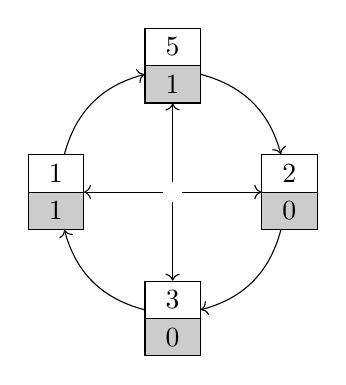
\begin{tikzpicture}[
        box/.style={
          draw,
          align=center,
          minimum width=2em,
          minimum height=6em,
          rectangle split,
          rectangle split parts=2,
          rectangle split part fill={white, black!20},
        }
      ]

        \node (c) at (0, 0) {};

        \node<1> [above=of c, box] (n) {0 \nodepart{second} 0};
        \node<2-5> [above=of c, box] {1 \nodepart{second} 1};
        \node<6-9> [above=of c, box] {1 \nodepart{second} 0};
        \node<10-> [above=of c, box] {5 \nodepart{second} 1};

        \node<1-2> [right=of c, box] (e) {0 \nodepart{second} 0};
        \node<3-6,11-12,16-> [right=of c, box] {2 \nodepart{second} 1};
        \node<7-10,13-15> [right=of c, box] {2 \nodepart{second} 0};

        \node<1-3> [below=of c, box] (s) {0 \nodepart{second} 0};
        \node<4-7,12-13,17-> [below=of c, box] {3 \nodepart{second} 1};
        \node<8-11,14-16> [below=of c, box] {3 \nodepart{second} 0};

        \node<1-4> [left=of c, box] (w) {0 \nodepart{second} 0};
        \node<5-8> [left=of c, box] (w) {4 \nodepart{second} 1};
        \node<9-14> [left=of c, box] (w) {4 \nodepart{second} 0};
        \node<15-> [left=of c, box] (w) {1 \nodepart{second} 1};

        \path [->] (n) edge [bend left] (e)
                   (e) edge [bend left] (s)
                   (s) edge [bend left] (w)
                   (w) edge [bend left] (n);

        \path<1,5,9,15-> [->] (c) edge (n);
        \path<2,6,10-12> [->] (c) edge (e);
        \path<3,7,13> [->] (c) edge (s);
        \path<4,8,14> [->] (c) edge (w);

      \end{tikzpicture}
    \end{center}

\end{slide}

\begin{slide}

    \slidetitle{Clock Example}

    Assume our physical memory can only hold 4 pages, and we access the following:

    \leftspace{}1 2 3 4 5 2 3 1 2 3 (all of the pages are initially on disk)

    \begin{center}
      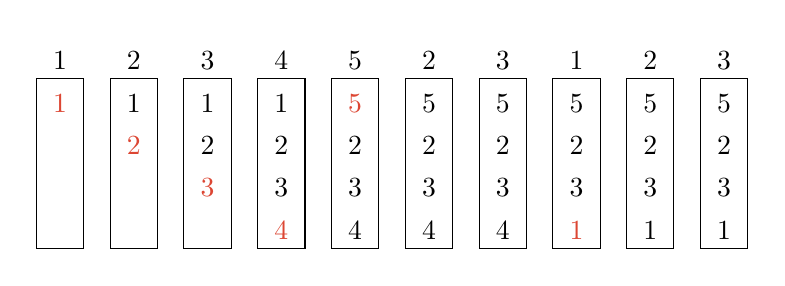
\begin{tikzpicture}[
        every node/.style={
          align=center,
          text height=2ex,
          text width=1em
        },
        swapin/.list={
          (2,1),
          (3,2),
          (4,3),
          (5,4),
          (2,5),
          (5,8)
        },
      ]
        \matrix (m) [
          matrix of nodes,
          nodes in empty cells,
          column sep=1em,
          column 2/.style={visible on=<2->},
          column 3/.style={visible on=<3->},
          column 4/.style={visible on=<4->},
          column 5/.style={visible on=<5->},
          column 6/.style={visible on=<6->},
          column 7/.style={visible on=<7->},
          column 8/.style={visible on=<8->},
          column 9/.style={visible on=<9->},
          column 10/.style={visible on=<10->},
        ] {
          1 & 2 & 3 & 4 & 5 & 2 & 3 & 1 & 2 & 3 \\
          1 & 1 & 1 & 1 & 5 & 5 & 5 & 5 & 5 & 5 \\
            & 2 & 2 & 2 & 2 & 2 & 2 & 2 & 2 & 2 \\
            &   & 3 & 3 & 3 & 3 & 3 & 3 & 3 & 3 \\
            &   &   & 4 & 4 & 4 & 4 & 1 & 1 & 1 \\
        };
        \draw (m-2-1.north west) rectangle (m-5-1.south east);
        \draw (m-2-2.north west) rectangle (m-5-2.south east);
        \draw (m-2-3.north west) rectangle (m-5-3.south east);
        \draw (m-2-4.north west) rectangle (m-5-4.south east);
        \draw (m-2-5.north west) rectangle (m-5-5.south east);
        \draw (m-2-6.north west) rectangle (m-5-6.south east);
        \draw (m-2-7.north west) rectangle (m-5-7.south east);
        \draw (m-2-8.north west) rectangle (m-5-8.south east);
        \draw (m-2-9.north west) rectangle (m-5-9.south east);
        \draw (m-2-10.north west) rectangle (m-5-10.south east);
      \end{tikzpicture}
    \end{center}

    \begin{flushright}
      \onslide<11->{6 page faults}
    \end{flushright}

\end{slide}

\begin{slide}

    \slidetitle{For Performance You May Choose to Disable Swapping}

    Memory is cheap, and has quite high capacity

    \leftspace{}You'd rather know you need more memory than run slowly

    \leftspace{}\leftspace{}Linux runs an OOM (out of memory) killer, that
    SIGKILLs the memory hog
    \medskip

    Larger page sizes allow for speedups (2 MiB or 1 GiB page size)

    \leftspace{}Trade more fragmentation for more TLB coverage

\end{slide}

\begin{slide}

    \slidetitle{The Clock Algorithm is an Approximation of LRU}

    Data structures:
    \begin{itemize}
      \item Keeps a circular list of pages in memory
      \item Uses a reference bit for each page in memory (light grey in next slides)
      \item Has a ``hand'' (iterator) pointing to the last element examined
    \end{itemize}
    \medskip

    Algorithm, to insert a new page:
    \begin{itemize}
      \item Check the hand's reference bit, if it's 0 then place the page and advance hand
      \item If the reference bit is 1, set it to 0, advance the hand, and repeat
    \end{itemize}
    \medskip

    For page accesses, set the reference bit to 1

\end{slide}
  
\end{document}
